\chapter{功能仿真结果}

\section{利用Chisel3配套工具进行快速仿真}
Chisel3在Github网站上有一套基于Scala体系的仿真工具,chisel-testers。
使用该工具可以直接在Scala中实例化使用Chisel3开发的模块,并且产生激励进行模块的仿真。
其主要提供了一个名为PeekPokeTester的类,该类提供了能够完成激励产生和信号断言的方法。
\begin{table}[h] %开始一个表格environment,表格的位置是h,here。  
    \centering
    \caption{PeekPokeTester中提供的方法} %显示表格的标题  
    \begin{tabular}{l|l|c} %设置了每一列的宽度,强制转换。  
    \hline  
    \hline  
    方法名 & 作用 & 使用举例 \\ %用&来分隔单元格的内容 \\表示进入下一行  
    \hline %画一个横线,下面的就都是一样了,这里一共有4行内容  
    poke & 设置DUT的输入信号 & poke(c.io.in.valid, 1) \\
    \hline  
    peek & 读取DUT的输出信号 & peek(c.io.out.bits) \\
    \hline  
    expect & 比较DUT的输出信号 & expect(c.io.out.bit, 0xff) \\
    \hline  
    step & 驱动DUT的时钟信号 & step(1) \\
    \hline
    reset & 驱动DUT的复位信号 & reset(1) \\
    \hline  
    \hline  
    \end{tabular}  
\end{table}
同时,该工具支持使用Verilator作为仿真后端,大大降低了大规模电路的仿真时间,借助Verilator,可以产生仿真时的vcd仿真文件,通过GTKWave、Verdi等波形查看工具即可查看仿真波形,
使用时十分便利。
            \begin{lstlisting}[title=Chisel Test Example, frame=shadowbox]
class Tester(c: Test) extends PeekPokeTester(c) {
  poke(c.io.in, -1)     //Set DUT input "in" as -1
  step(1)               //wait 1 clock
  expect(c.io.out, -1)  //assert DUT output "out" as -1
}
            \end{lstlisting}

\section{基于FIFO的可变长移位寄存器仿真结果}
% filters: DenseVector(0, 2, -1) __ 3
% filterNum: 1
% imgs: DenseVector(4, -3, -3, -1, -5) __ 5
% imgNum: 1
% nchannel: 1
\begin{figure}[h]
    \centering
    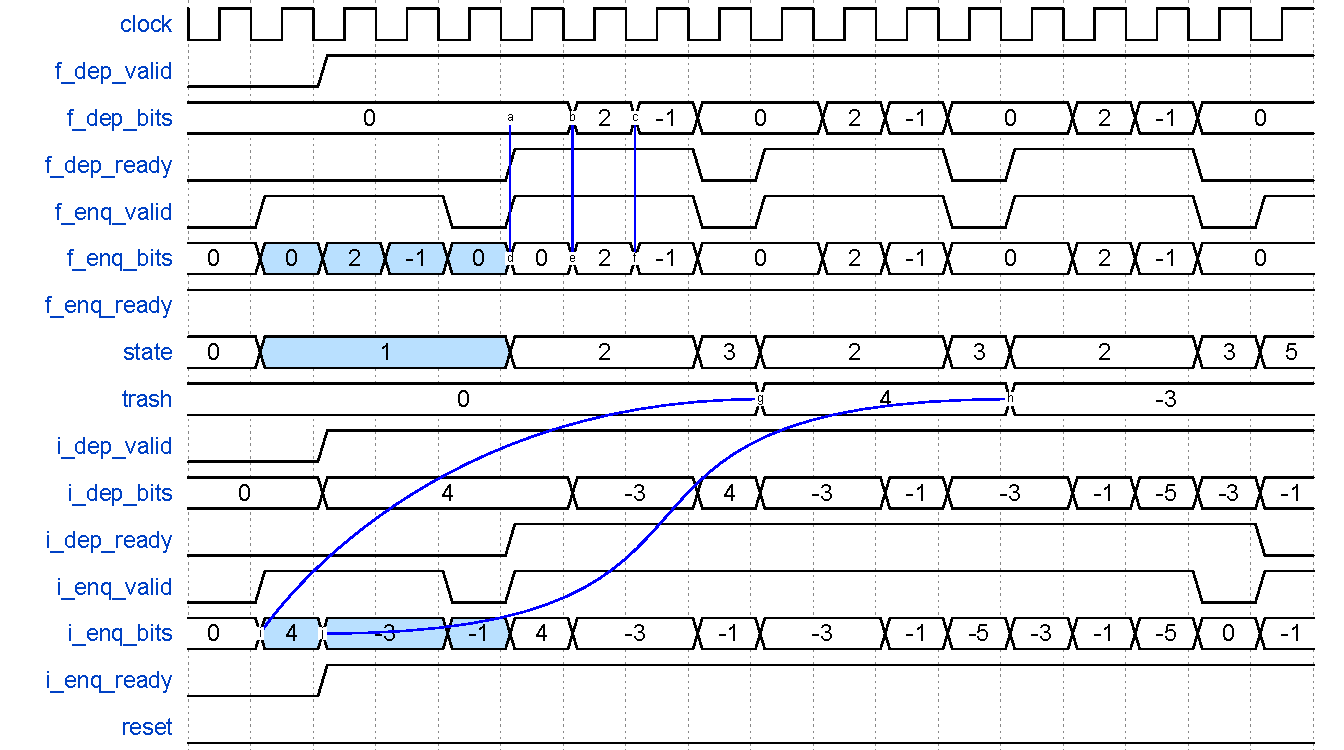
\includegraphics[scale=0.7]{../pdf/shift_w.pdf}\\
    \caption{SRAM IP波形图}
\end{figure}

\section{Designware SRAM IP仿真结果}
\begin{figure}[h]
    \centering
    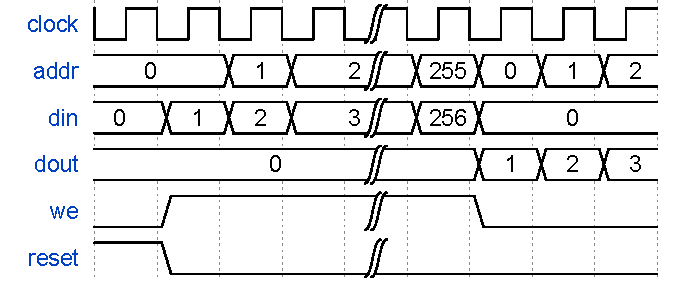
\includegraphics{../pdf/sram_w.pdf}\\
    \caption{SRAM IP波形图}
\end{figure}

\section{PE单元仿真结果}

\section{PE阵列仿真结果}

\section{运行MNIST测试结果}
    \subsection{模型量化}
    \subsection{运行流程}
    \subsection{输出结果与数学结果映射关系}

\section{系统性能}
    \subsection{资源占用}
    \subsection{时序报告}

\section{本章小结}
% \subsection{二级节标题}

% \subsubsection{三级节标题}

% \paragraph{四级节标题}

% \subparagraph{五级节标题}

% \section{脚注}

% Lorem ipsum dolor sit amet, consectetur adipiscing elit, sed do eiusmod tempor
% incididunt ut labore et dolore magna aliqua. Ut enim ad minim veniam, quis
% nostrud exercitation ullamco laboris nisi ut aliquip ex ea commodo consequat.
% Duis aute irure dolor in reprehenderit in voluptate velit esse cillum dolore eu
% fugiat nulla pariatur. Excepteur sint occaecat cupidatat non proident, sunt in
% culpa qui officia deserunt mollit anim id est laborum.
% \footnote{This is a long long long long long long long long long long long long
% long long long long long long long long long long footnote.}
